\documentclass[12pt]{article}

\usepackage{amsmath}
\usepackage{amssymb}
\usepackage{geometry}
\usepackage{graphicx}
\usepackage{hyperref}

\geometry{letterpaper,tmargin=1in,bmargin=1in,lmargin=1in,rmargin=1in}

\hypersetup{
colorlinks, linkcolor=blue,
}


\begin{document}

\title{Analog IC Design: Project - Part 2}
\date{Spring 2018}
\maketitle
\tableofcontents

\newpage
\section{Objective}

In part 1 of this project we designed a Operational-Amplifier from scratch. This was done by following a step by step incremental process. This allows for the understanding of each component of the circuit before moving forward to more complicated steps. In continuation of that theme we are going to take that previously constructed circuit and cascade it to increase its overall gain. After that is accomplished we will then attempt to cascade it again but with a single ended output.

\subsection{Primary Tasks}
The purpose of this project can be simplified into to primary tasks as given.
\begin{enumerate}
	\item Determining the biasing circuit configuration
	\item Designing/calculate all the MOSFETs parameters to achieve the desired amplifier
	specifications.
\end{enumerate}

\subsection{Circuit Requirements}
The following are given circuit requirements that will be adhered to.

\begin{enumerate}
	\item Do whatever modifications necessary to your circuit in the first part to cascode the
	differential stage, as shown in figure 9.13(a) in the textbook.
	\item The new differential gain should be equal to 104
	(with a tolerance of no more than
	20\%, but the gain should be at least 104
	)
	\item Allowed 1 resistor (to be placed outside the IC), any number of n-type and
	p-type enhancement mode MOSFETS.
	\item Allowed a maximum of 2 power supplies (excluding the test input signal source
	of course)
	\item $\lambda$ for all MOSFETS should be at least 0.02
	\item W and L should be at least 1µm (assuming a 1µm technology).
\end{enumerate}


\subsection{Custom MOSFETS}
\label{sec:desigan_and_analysis}

We will be using the MOSFETs that were designated in part one of the project. They are as follows

\begin{itemize}
	\item NMOS \newline \newline
	.SUBCKT enmos001 1 2 3 \newline
	M 1 2 3 3 enmos001\newline
	.MODEL enmos001 NMOS (KP = 500E-6 VTO = 1 LAMBDA = 0.02 W=2u L=1u)\newline
	.ENDS enmos001
\newline
	\item PMOS \newline \newline
	.SUBCKT enmos002 1 2 3 \newline
	M 1 2 3 3 enmos002\newline
	.MODEL enmos002 PMOS (KP = 500E-6 VTO = 1 LAMBDA = 0.02 W=2u L=1u)\newline
	.ENDS enmos002
\newline
	
\end{itemize}

Using Multisim's component wizard we can import this settings and create custom MOSFETs for use in our simulation.

\subsubsection{Problems Encountered}
In part one of the project the above MOSFETs where causing wild variations in readings, switching to Multisim 14 helped to solved those problems. Multisim 14 was also used in part two of the project to prevent further issues.


\section{Initial Circuit}
The design that I designed in the previous project is as follows. The sections are colored to show the purpose of each area of the circuit. This is the circuit that will be cascoded for this project.


\begin{figure}[h!]
	\label{fig:amp}
	\caption{Project: Part 1}
	\centering
	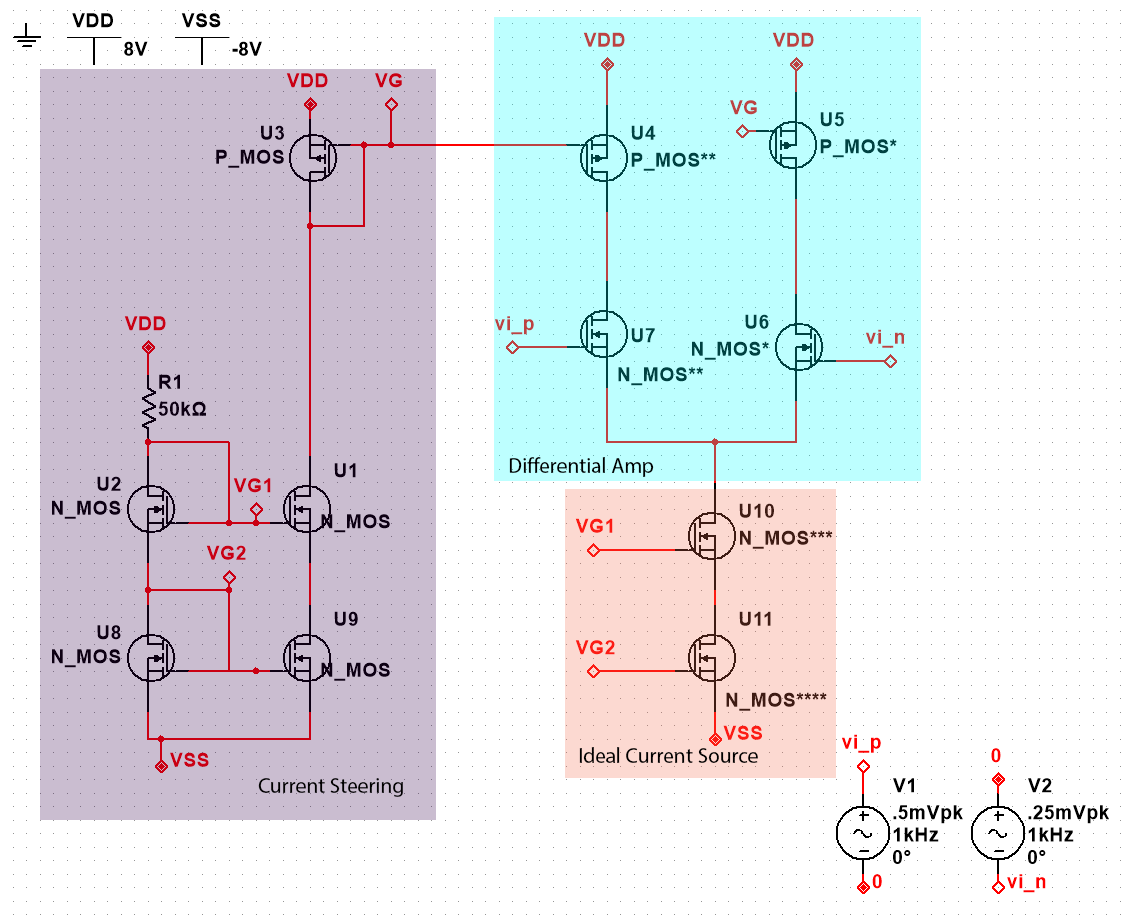
\includegraphics[width=.6\textwidth]{photoshop}
\end{figure}



\subsection{Analysis}
The analysis of the designed circuit shows that a gain of $100$ is being obtained. This is at Probe 1 in reference to Probe 4. For our doubled ended cascoded amplifier we will be aiming for a gain of $10000$

\begin{figure}[h!]
	\label{fig:amp}
	\caption{Final Circuit Analysis}
	\centering
	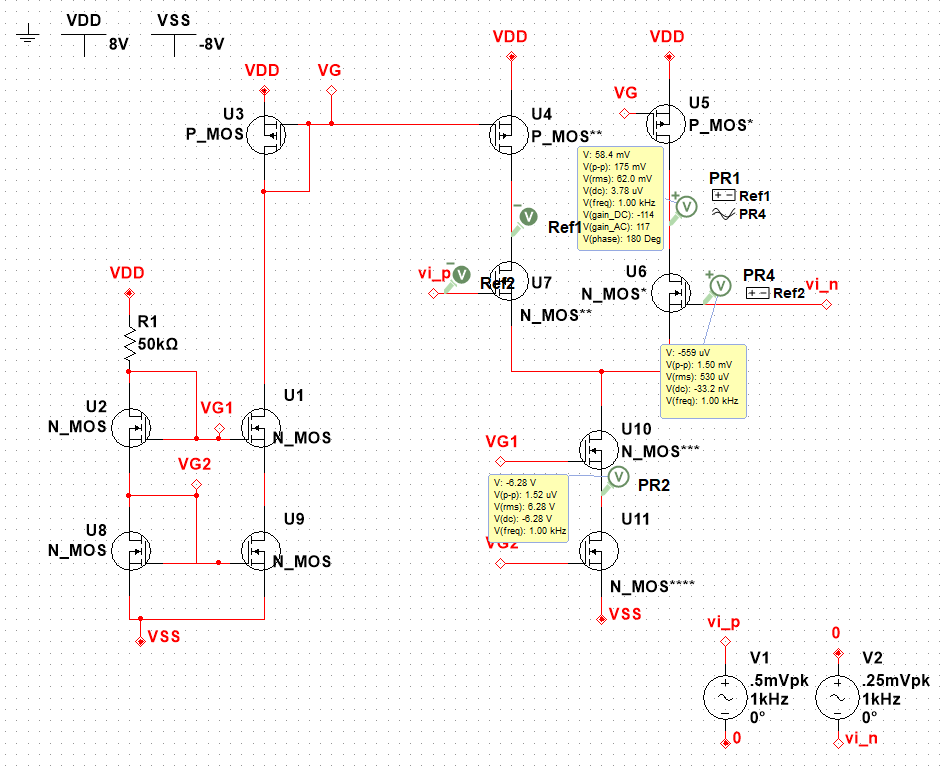
\includegraphics[width=1\textwidth]{finalamp}
\end{figure}


\section{Double ended Cascoded Amplifier}
For our amplifier to work in a cascoded configuration we must calculate several values, including biasing voltages, drain current, and a new resistance value.
\subsection{Gain Equation}
Be fore we can start solving for other parts of the circuit we need to go ahead and find a equation for the gain of our circuit. From the book we can see that the gain can be obtained by the differential-half circuit of the cascoded amplifier, it is as follows

$$A_d \equiv \frac{V_{od}}{V_{id}} = g_{m1} (R_{on}|| R_{op})$$

where
 $$R_{on} = (g_{m3} R_{o3}) R_{o1}$$ 
and 
$$R_{op} = (g_{m5} R_{o5}) R_{o7}$$

with those equations and our equation for transconductance 
$$g_{m} = \sqrt{2 K_n I_D}$$
 we can begin to solve for $A_D$
 
$$R_{on} =\frac{1}{\lambda I_D} \frac{1}{\lambda I_D} g_m$$
$$R_{on} = \frac{1}{\lambda^2 I_D^2} g_m$$
$$R_{on} = \frac{1}{\lambda^2 I_D^2} \sqrt{2 K_n I_D}$$
$$R_{on}|| R_{op} = \frac{1}{2} \frac{1}{\lambda^2 I_D^2} \sqrt{2 K_n I_D}  $$

Now we take $R_{on}|| R_{op}$ and plug it into our gain equation $A_d \equiv \frac{V_{od}}{V_{id}} = g_{m1} (R_{on}|| R_{op})$


$$A_d = \frac{1}{2} \frac{1}{\lambda^2 I_D^2} \sqrt{2 K_n I_D} \sqrt{2 K_n I_D}$$
 which simplifies to our gain equation,
 
$$A_d  = \frac{K_n}{\lambda^2 I_D}$$
 
\subsection{Calculating Drain Current $I_d$}
With the given constants $K_n = K_p = .5m$ and $\lambda = .02$ we can effectively solve for $I_D$ using the gain equation and $A_d = 10000$

$$A_d  = \frac{K_n}{\lambda^2 I_D}$$
 


$$I_D = 250\mu A$$
 
\section{Conclusion}
The project so far has been challenging but rewarding. In terms of progress so far, by chopping the assignment into pieces and individual circuits it made tackling the final circuit that much easier. The Differential amplifier using the given transistors does in fact work, which on its own is very satisfying. I look forward to continuing and completing the design.





\end{document}
